\documentclass[12pt,a4paper]{article}
\usepackage[utf8]{inputenc}
\usepackage[english]{babel}
\usepackage{geometry}
\geometry{left=2cm,right=2cm,top=2cm,bottom=2cm}
\usepackage{graphicx}
\usepackage{hyperref}
\hypersetup{
    colorlinks=true,
    linkcolor=blue,
    urlcolor=blue,
}
\usepackage{tikz}
\usetikzlibrary{positioning,arrows,calc,shapes}
\usepackage{listings}
\usepackage{xcolor}
\usepackage{amsmath}
\usepackage{enumitem}
\usepackage{fancyhdr}
\usepackage{lastpage}
\usepackage{tikz}
\usetikzlibrary{positioning, arrows, calc, shapes, shadows, decorations.pathmorphing}
\pagestyle{fancy}
\fancyhf{}
\fancyhead[L]{OAuth 2.0 Penetration Testing Notes}
\fancyhead[R]{\thepage/\pageref{LastPage}}
\renewcommand{\headrulewidth}{0.4pt}

\definecolor{codebg}{rgb}{0.95,0.95,0.95}
\lstdefinestyle{httpstyle}{
    backgroundcolor=\color{codebg},
    basicstyle=\ttfamily\small,
    breaklines=true,
    tabsize=4,
    showstringspaces=false,
    frame=single,
    captionpos=b,
    xleftmargin=10pt,
    xrightmargin=10pt
}
\lstset{style=httpstyle}

% TikZ styles for sequence diagrams
\tikzset{
    actor/.style={
        rectangle,
        draw,
        fill=blue!10,
        minimum width=1.5cm,
        minimum height=0.8cm,
        align=center,
        rounded corners
    },
    arrow/.style={
        ->,
        >=stealth',
        thick
    },
    note/.style={
        draw,
        dashed,
        fill=yellow!20,
        align=left,
        font=\small
    }
}

\title{\Huge \textbf{OAuth 2.0 Authentication} \\[0.5cm]
\Large Penetration Testing Notes}
\author{\textbf{Eyad Islam El-Taher}}
\date{\today}

\begin{document}

\maketitle
\thispagestyle{empty}
\newpage

\tableofcontents
\newpage

\section{Introduction}
OAuth 2.0 is an authorization framework that enables third-party applications to obtain limited access to a user's resources without exposing their credentials. While the protocol itself is robust, real-world implementations often introduce vulnerabilities that attackers can exploit. This document provides a comprehensive guide for penetration testers to understand OAuth internals, identify weaknesses, and perform offensive assessments.

\subsection{Why OAuth Matters for Pentesters}
\begin{itemize}
    \item OAuth is the backbone of modern authentication (SSO, social login, API protection).
    \item Implementation flaws are common and often critical, leading to account takeover.
    \item OAuth tokens and codes are valuable targets; attackers aim to steal them.
    \item The attack surface is broad: redirect URIs, state parameters, scope validation, client secrets, etc.
\end{itemize}

This guide covers:
\begin{itemize}
    \item OAuth fundamentals and components.
    \item Detailed explanation of flows (Authorization Code, Implicit, etc.).
    \item Common vulnerabilities with step-by-step exploitation.
    \item Detection and prevention methodologies.
    \item Real-world examples and PortSwigger labs walkthroughs.
\end{itemize}

\section{OAuth Fundamentals}
\subsection{Core Concepts}
OAuth decouples authentication from authorization. The user (Resource Owner) authenticates with the Authorization Server (IdP) and grants permission to the Client Application to access resources on the Resource Server.

\subsection{OAuth Components}
\begin{itemize}
    \item \textbf{Resource Owner} – The user who owns the data and consents to access.
    \item \textbf{Client Application} – The application requesting access (e.g., a web or mobile app).
    \item \textbf{Authorization Server} – Issues tokens after authenticating the user and obtaining consent.
    \item \textbf{Resource Server} – Hosts the protected resources (APIs) that the client wants to access.
    \item \textbf{Identity Provider (IdP)} – Often integrated with the Authorization Server; authenticates the user.
    \item \textbf{User Agent} – The browser or native application used by the resource owner.
\end{itemize}

\subsection{OAuth Endpoints}
\vspace*{0.25cm}
\begin{table}[h]
\centering
\begin{tabular}{|p{3cm}|p{4cm}|p{2cm}|p{7cm}|}
\hline
\textbf{Endpoint} & \textbf{Purpose} & \textbf{Method} & \textbf{Key Parameters} \\
\hline
\texttt{/authorize} & Initiates the OAuth flow & GET & \texttt{client\_id},\texttt{redirect\_uri}, \texttt{response\_type}, \texttt{scope}, \texttt{state} \\
\hline
\texttt{/token} & Exchanges code for tokens & POST & \texttt{grant\_type}, \texttt{code}, \texttt{client\_id}, \texttt{client\_secret} \\
\hline
\texttt{/userinfo} & Returns user data & GET & \texttt{Authorization: Bearer <token>} \\
\hline
\texttt{/introspection} & Validates token status & POST & \texttt{token} \\
\hline
\texttt{/revoke} & Revokes a token & POST & \texttt{token} \\
\hline
\end{tabular}
\caption{OAuth Endpoints}
\end{table}

\subsection{OAuth Tokens}
\begin{itemize}
    \item \textbf{Access Token} – Used to access resources. Short-lived (minutes to hours). Stored client-side. Validated by Resource Server.
    \item \textbf{Refresh Token} – Used to obtain new access tokens. Long-lived. Stored by the client (secured). Validated by Authorization Server.
    \item \textbf{Authorization Code} – Temporary code exchanged for tokens. Single-use, short-lived. Sent to client via redirect.
    \item \textbf{ID Token} – JSON Web Token (JWT) containing user identity claims. Used in OpenID Connect.
    \item \textbf{Bearer Token} – Any token that can be used as a bearer credential (e.g., in \texttt{Authorization} header).
\end{itemize}

\section{OAuth Flows}
\subsection{Authorization Code Grant}
\paragraph{Overview} The most secure flow. The client obtains an authorization code via user consent, then exchanges it for an access token through a back-channel (server-to-server) request.

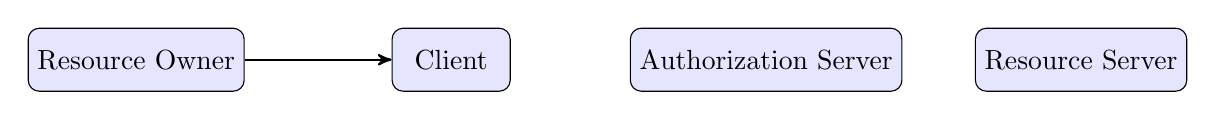
\begin{tikzpicture}[node distance=4cm, auto]
    \node[actor] (user) {Resource Owner};
    \node[actor, right of=user] (client) {Client};
    \node[actor, right of=client] (auth) {Authorization Server};
    \node[actor, right of=auth] (resource) {Resource Server};

    \draw[arrow] (user) -- node[above, rotate=90, anchor=south] {} (client);
    % We'll use a more detailed diagram later
\end{tikzpicture}

\paragraph{Steps:}
\begin{enumerate}
    \item Client redirects user to Authorization Server with \texttt{response\_type=code}.
    \item User authenticates and consents.
    \item Authorization Server redirects back with an authorization code.
    \item Client exchanges code for access token (using client secret).
    \item Authorization Server returns access token (and optionally refresh token).
    \item Client uses access token to access Resource Server.
\end{enumerate}

\subsection{Implicit Grant}
\paragraph{Overview} Used for public clients (e.g., SPA). The access token is returned directly in the redirect URI fragment. Less secure because token is exposed in the browser.

\subsection{Other Flows}
\begin{itemize}
    \item \textbf{Resource Owner Password Credentials} – Directly sends user credentials to client (not recommended).
    \item \textbf{Client Credentials} – Machine-to-machine communication using client secret only.
\end{itemize}

\section{Common Misconceptions}
\begin{itemize}
    \item OAuth is not authentication; it's authorization. OpenID Connect adds authentication.
    \item The client secret is not needed for public clients (SPAs, mobile apps) because it can't be kept secret.
    \item The \texttt{state} parameter is not optional; it protects against CSRF.
    \item The \texttt{redirect\_uri} must be strictly validated; domain-only validation is insufficient.
    \item Implicit flow is deprecated for new applications; use Authorization Code with PKCE.
\end{itemize}

\section{Attack Surface}
The OAuth attack surface includes:
\begin{itemize}
    \item \textbf{Redirect URI} – Manipulation leads to code/token leakage.
    \item \textbf{State Parameter} – Missing or predictable leads to CSRF.
    \item \textbf{Scope Parameter} – Flawed validation allows privilege escalation.
    \item \textbf{Client Secret} – Exposure (e.g., in source code) leads to token theft.
    \item \textbf{Authorization Code} – Leakage via referer headers, open redirects, or postMessage.
    \item \textbf{Access Token} – Leakage via browser history, logs, or JavaScript.
    \item \textbf{Account Linking} – Flaws allow attackers to associate malicious accounts.
    \item \textbf{User Registration} – Unverified email allows account takeover.
\end{itemize}

\section{OAuth Vulnerabilities}
\subsection{Authentication Bypass via OAuth Implicit Flow}
\subsubsection{Theory}
In the implicit flow, the access token is returned in the URL fragment. If the client application does not properly validate the token's origin or audience, an attacker can trick the client into using a token issued for a different application or user.

\subsubsection{Why It Happens}
The client application trusts the token without verifying its intended audience (\texttt{aud} claim) or signature, or it accepts tokens from any authorization server.

\subsubsection{Attack Prerequisites}
\begin{itemize}
    \item Victim uses an OAuth client that accepts tokens from a configured issuer.
    \item Attacker can obtain an access token for their own account from the same or a different OAuth provider.
    \item The client does not validate the token's audience or issuer properly.
\end{itemize}

\subsubsection{Step-by-Step Exploitation}
\begin{enumerate}
    \item Attacker registers an application with the OAuth provider and obtains an access token for their own account.
    \item Attacker intercepts the redirect URI of the victim client and replaces the token with their own.
    \item The victim client accepts the token and logs the attacker in as the victim.
\end{enumerate}

\subsubsection{HTTP Request Example}
\begin{lstlisting}
GET /callback#access_token=attacker_token&token_type=Bearer
\end{lstlisting}


\subsubsection{Real-World Scenario}
A single-page application using implicit flow accepts any token from a trusted provider without checking the \texttt{aud} claim. An attacker obtains a token for a different app and uses it to log in.

\subsubsection{Impact}
Account takeover, privilege escalation.

\subsubsection{Detection Methodology}
\begin{itemize}
    \item Check if the client validates the token's \texttt{iss} and \texttt{aud} claims.
    \item Attempt to use a token issued for a different client ID.
    \item Use Burp to intercept and replace tokens in redirects.
\end{itemize}


\subsubsection{Important Notes}
\begin{itemize}
    \item Implicit flow is deprecated; many modern apps use Authorization Code with PKCE, which mitigates this.
\end{itemize}

% ---------------------------------------------------------------------
\subsection{Improper \texttt{redirect\_uri} Validation}
\subsubsection{Theory}
The \texttt{redirect\_uri} parameter determines where the authorization code/token is sent. If the Authorization Server does not strictly validate the URI (e.g., only checks the domain), attackers can redirect the code to a malicious endpoint.

\subsubsection{Why It Happens}
Developers often use loose validation (e.g., domain match or prefix match) to allow flexibility, but this opens the door to open redirect and code leakage.

\subsubsection{Attack Prerequisites}
\begin{itemize}
    \item The Authorization Server does not enforce exact URI matching.
    \item The client application has registered a URI that can be manipulated via path traversal or subdomain tricks.
\end{itemize}

\subsubsection{Step-by-Step Exploitation (Path Traversal)}
\begin{enumerate}
    \item Find a whitelisted domain, e.g., \texttt{https://app.com/oauth-callback}.
    \item Construct a malicious \texttt{redirect\_uri} that uses path traversal to redirect to an open redirect endpoint: \\
    \texttt{https://app.com/oauth-callback/../post/next?path=https://attacker.com}.
    \item If the server allows that, the authorization code will be sent to \texttt{https://attacker.com} via the open redirect.
    \item Attacker logs the code and uses it.
\end{enumerate}

\subsubsection{HTTP Request Example}
\begin{lstlisting}
GET /auth?client_id=123&redirect_uri=https://app.com/oauth-callback/../post/next?path=https://attacker.com&response_type=code
\end{lstlisting}

\subsubsection{Attack Diagram}
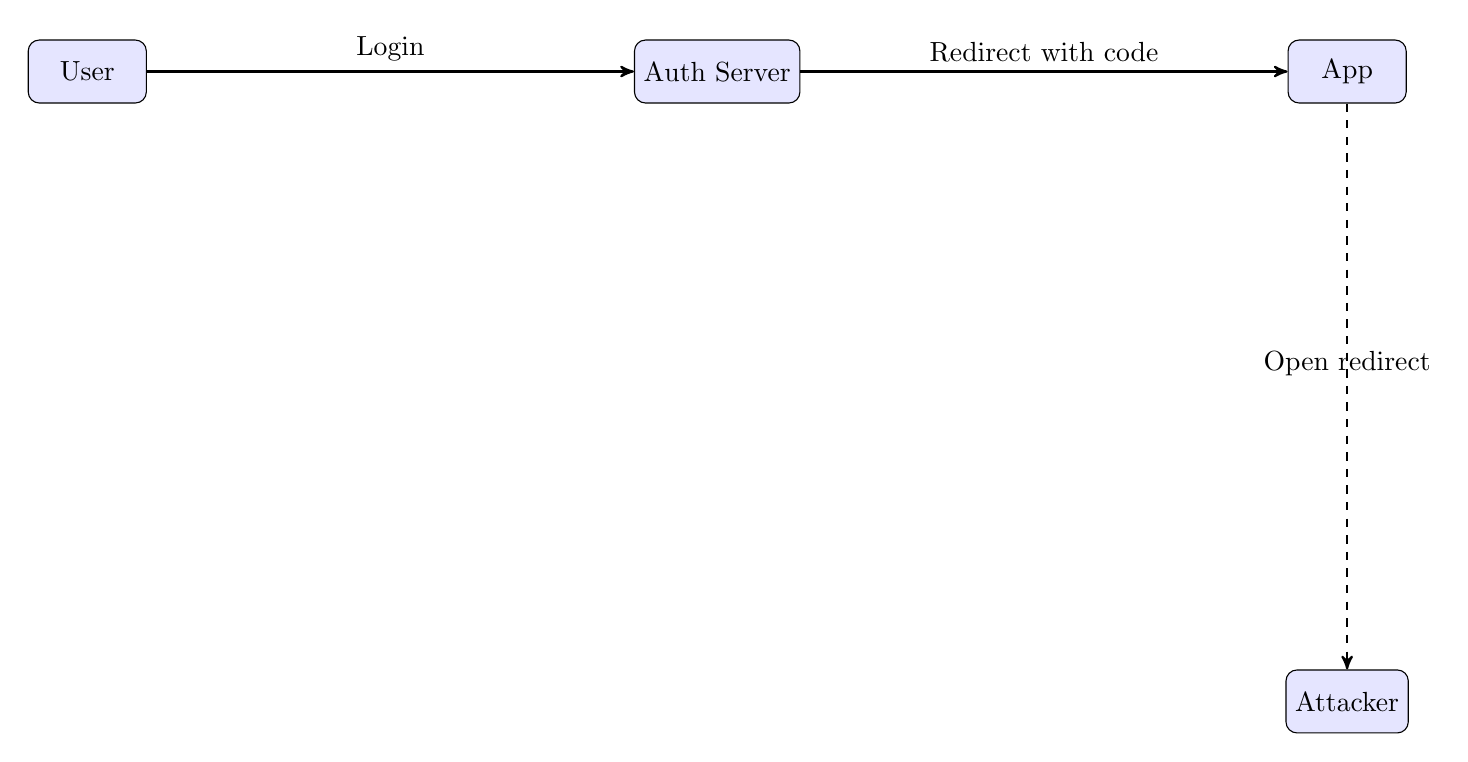
\begin{tikzpicture}[node distance=8cm, auto]
    \node[actor] (user) {User};
    \node[actor, right of=user] (auth) {Auth Server};
    \node[actor, right of=auth] (app) {App};
    \node[actor, below of=app] (attacker) {Attacker};
    \draw[arrow] (user) -- node[above] {Login} (auth);
    \draw[arrow] (auth) -- node[above] {Redirect with code} (app);
    \draw[arrow, dashed] (app) -- node[above] {Open redirect} (attacker);
\end{tikzpicture}


\subsubsection{Impact}
Authorization code leakage, account takeover.

\subsubsection{Detection Methodology}
\begin{itemize}
    \item Try to modify \texttt{redirect\_uri} to a domain you control.
    \item Test for path traversal, open redirect chaining, and subdomain takeover.
    \item Observe if the Authorization Server redirects with a code.
\end{itemize}

\subsubsection{Burp Suite Methodology}
\begin{enumerate}
    \item Intercept the \texttt{/authorize} request.
    \item Change \texttt{redirect\_uri} to various malicious values.
    \item Send and follow redirects to see if code is leaked.
\end{enumerate}

\subsubsection{Prevention}
\begin{itemize}
    \item Use exact URI matching (including path and query).
    \item Maintain a whitelist of full redirect URIs.
    \item Normalize URIs before comparison.
\end{itemize}

\subsubsection{Pentesting Tips}
\begin{itemize}
    \item Use Burp's \textit{Intruder} to fuzz the \texttt{redirect\_uri} with common bypass strings.
    \item Look for open redirect parameters on the client application to chain.
\end{itemize}


% ---------------------------------------------------------------------
\subsection{Missing \texttt{state} Parameter (CSRF)}
\subsubsection{Theory}
The \texttt{state} parameter is used to prevent CSRF attacks by binding the authorization request to the user's session. If missing or predictable, an attacker can initiate a flow and force a victim to complete it, linking the attacker's account to the victim's.

\subsubsection{Why It Happens}
Developers overlook the \texttt{state} parameter or consider it optional.

\subsubsection{Attack Prerequisites}
\begin{itemize}
    \item Authorization Server does not require \texttt{state}.
    \item The client application does not verify it on callback.
\end{itemize}

\subsubsection{Step-by-Step Exploitation (Account Linking)}
\begin{enumerate}
    \item Attacker initiates OAuth flow with their own account, copying the authorization URL.
    \item Attacker modifies the \texttt{redirect\_uri} (if possible) or uses an iframe to force the victim to complete the flow.
    \item Victim is redirected and authenticates; the authorization code is sent to the attacker's \texttt{redirect\_uri} (if not validated) or the attacker's session is used.
    \item If the code is sent to the attacker-controlled endpoint, they can exchange it and link the victim's account to their social profile.
\end{enumerate}

\subsubsection{HTTP Request Example}
\begin{lstlisting}
GET /auth?client_id=123&redirect_uri=https://attacker.com&response_type=code
\end{lstlisting}


\subsubsection{Impact}
Account takeover, unauthorized linking of accounts.

\subsubsection{Detection Methodology}
\begin{itemize}
    \item Check the \texttt{/authorize} request for a \texttt{state} parameter.
    \item If present, test if it's predictable (e.g., fixed value, session ID).
    \item Attempt to initiate the flow without \texttt{state} and see if it succeeds.
\end{itemize}

\subsubsection{Burp Suite Methodology}
\begin{enumerate}
    \item Intercept the authorization request.
    \item Remove or modify the \texttt{state} parameter.
    \item Observe if the callback still works and if the session is hijacked.
\end{enumerate}

\subsubsection{Prevention}
\begin{itemize}
    \item Always generate a cryptographically random \texttt{state} and validate it on callback.
    \item Bind \texttt{state} to the user's session.
\end{itemize}


\subsubsection{Pentesting Tips}
\begin{itemize}
    \item Try to brute-force predictable \texttt{state} values.
    \item Use Burp's CSRF token analysis features.
\end{itemize}

\subsubsection{Important Notes}
\begin{itemize}
    \item Even if \texttt{state} is present, check if it's validated correctly.
\end{itemize}

% ---------------------------------------------------------------------
\subsection{Flawed Scope Validation}
\subsubsection{Theory}
The scope parameter defines the permissions requested. If the Authorization Server does not validate the scope during the token exchange against the originally approved scope, an attacker can upgrade the token's permissions.

\subsubsection{Why It Happens}
The token endpoint may ignore the scope from the authorization step and accept a new scope in the token request.

\subsubsection{Attack Prerequisites}
\begin{itemize}
    \item The attacker controls a client application (can modify token exchange request).
    \item The Authorization Server does not enforce scope consistency.
\end{itemize}

\subsubsection{Step-by-Step Exploitation}
\begin{enumerate}
    \item Client requests authorization with a limited scope (e.g., \texttt{openid email}).
    \item User approves.
    \item Client exchanges authorization code for token, adding a broader scope (e.g., \texttt{openid email profile}) in the POST to \texttt{/token}.
    \item If the server doesn't validate against the original approved scope, it returns a token with the broader scope.
\end{enumerate}

\subsubsection{HTTP Request Example}
\begin{lstlisting}
POST /token
Host: auth-server.com
Content-Type: application/x-www-form-urlencoded

client_id=123&client_secret=secret&grant_type=authorization_code&code=abc&redirect_uri=https://app.com&scope=openid%20email%20profile
\end{lstlisting}


\subsubsection{Impact}
Privilege escalation, unauthorized data access.

\subsubsection{Detection Methodology}
\begin{itemize}
    \item Capture the token exchange request and modify the \texttt{scope} parameter.
    \item Observe if the returned token grants the expanded scope.
\end{itemize}

\subsubsection{Burp Suite Methodology}
\begin{enumerate}
    \item Intercept the \texttt{/token} request.
    \item Add or modify the \texttt{scope} parameter.
    \item Forward and test the new token's permissions.
\end{enumerate}

\subsubsection{Prevention}
\begin{itemize}
    \item Always validate that the requested scope does not exceed the originally approved scope.
    \item Store the approved scope with the authorization code and enforce it.
\end{itemize}
 
\subsubsection{Pentesting Tips}
\begin{itemize}
    \item Test all scopes that the client might support.
\end{itemize}


% ---------------------------------------------------------------------
\subsection{Unverified User Registration}
\subsubsection{Theory}
If the OAuth provider allows registration without email verification, an attacker can create an account with the victim's email address. When the victim later tries to log in using that provider, the client may associate the attacker's account with the victim.

\subsubsection{Why It Happens}
The root cause is insufficient identity verification during the registration process:
\begin{itemize}
    \item \textbf{No email verification} - The OAuth provider doesn't send a confirmation email or require clicking a verification link
    \item \textbf{Trusting unverified data} - Client applications blindly trust the email claim from the OAuth provider
    \item \textbf{Using email as unique identifier} - Applications use email as the primary key instead of the OAuth provider's unique \texttt{sub} (subject) identifier
\end{itemize}


\subsubsection{Step-by-Step Exploitation}
\paragraph{Phase 1: Pre-Registration (Attacker Prepares)}
\begin{enumerate}
    \item Attacker identifies victim's email address (e.g., \texttt{victim@company.com})
    \item Attacker goes to OAuth provider's signup page
    \item Attacker registers using victim's email without verification
    \item Provider creates the account since email verification is not required
    \item Attacker now "owns" that email address in the OAuth provider's system
\end{enumerate}

\paragraph{Phase 2: The Attack}
\begin{enumerate}
    \item Victim visits a third-party application
    \item Victim clicks "Login with [OAuth Provider]"
    \item OAuth flow starts - Victim is redirected to the OAuth provider
    \item Victim tries to log in (if they have a real account, they might be blocked)
    \item Client application receives the user's data from the OAuth provider
    \item Application checks the email - it sees \texttt{victim@company.com}
    \item Application looks up the user in its database using that email
    \item If the attacker already linked this email to an account in the app, the victim might be logged into the attacker's account
\end{enumerate}

\subsubsection{Attack Scenarios}
Scenario 1: Pre-emptive Account Takeover
\begin{lstlisting}
Timeline:
Day 1: Attacker registers with victim@company.com on OAuth provider
       (no email verification required)
       -->
Day 1: Attacker uses that OAuth account to log into target app
       Target app creates account with victim@company.com
       -->
Day 2: Victim tries to log in using same OAuth provider
       Target app finds existing account (created by attacker)
       Victim is now in the attacker's account!
\end{lstlisting}

Scenario 2: Denial of Service
\begin{lstlisting}
Day 1: Attacker registers with victim@company.com
       -->
Day 2: Victim tries to register with same OAuth provider
       Provider says: "Email already in use"
       Victim cannot use this OAuth provider at all
\end{lstlisting}

Scenario 3: Account Linking Confusion
\begin{lstlisting}
Day 1: Victim already has an account on target app (password-based)
       -->
Day 2: Attacker registers with victim@company.com on OAuth provider
       -->
Day 3: Victim tries to "Link Social Account" feature
       Victim logs in with OAuth provider
       Target app sees email matches existing account
       But OAuth account belongs to attacker (same email)
       Now attacker's OAuth account is linked to victim's app account!
       -->
Day 4: Attacker logs in using their OAuth account
       Since it's linked to victim's app account, attacker is now logged in as victim!
\end{lstlisting}


\subsubsection{Impact}
\begin{table}[h]
\centering
\begin{tabular}{|c|l|}
\hline
\textbf{Impact Level} & \textbf{Description} \\
\hline
\textcolor{red}{Critical} & Complete account takeover \\
\textcolor{orange}{High} & Ability to impersonate victim \\
\textcolor{yellow}{Medium} & Denial of service (victim can't use OAuth) \\
\hline
\end{tabular}
\end{table}

\subsubsection{Detection Methodology}
\paragraph{Manual Testing Steps:}
\begin{enumerate}
    \item \textbf{Check OAuth provider registration}
    \begin{itemize}
        \item Try to register with a disposable email
        \item See if you receive a verification email
        \item Try to log in without verifying
    \end{itemize}
    
    \item \textbf{Test account takeover}
    \begin{itemize}
        \item Register with victim's email (if you control it or it's public)
        \item Try to use that account on target application
    \end{itemize}
    
    \item \textbf{Check \texttt{email\_verified} claim}
    \begin{itemize}
        \item Intercept OAuth response
        \item Look for \texttt{email\_verified} field in the userinfo response
    \end{itemize}
    
    \item \textbf{Test target application's behavior}
    \begin{itemize}
        \item Does it check \texttt{email\_verified} claim?
        \item Does it use \texttt{sub} or \texttt{email} as the unique identifier?
    \end{itemize}
\end{enumerate}

\subsubsection{Prevention}
\paragraph{For OAuth Providers:}
\begin{itemize}
    \item Always verify email addresses before allowing account creation
    \item Send verification email with a token/link
    \item Mark accounts as unverified until verification is complete
    \item Don't allow login with unverified email
    \item Support \texttt{email\_verified} claim in userinfo endpoint
\end{itemize}

\paragraph{For Client Applications:}
\begin{itemize}
    \item Use \texttt{sub} (subject) as unique identifier, NOT email
    \item Check \texttt{email\_verified} claim if available
    \item Require additional verification for sensitive actions
    \item Implement step-up authentication for high-risk users
    \item Don't automatically link accounts based on email alone
\end{itemize}


\subsubsection{Pentesting Tips}
\begin{enumerate}
    \item \textbf{Test registration without verification}
    \begin{lstlisting}
Register -> Check email -> No email received -> Login works?
    \end{lstlisting}
    
    \item \textbf{Test email takeover}
    \begin{lstlisting}
Register with victim@domain.com -> Use that account -> Victim can't register
    \end{lstlisting}
    
    \item \textbf{Check OAuth userinfo response}
    \begin{lstlisting}
GET /userinfo -> Look for email_verified -> If missing or false, test further
    \end{lstlisting}
    
    \item \textbf{Test account linking}
    \begin{lstlisting}
Try to link OAuth account to an existing account -> What happens?
    \end{lstlisting}
\end{enumerate}


% ---------------------------------------------------------------------
\subsection{Access Token Leakage via Open Redirect}
\subsubsection{Theory}
If the \texttt{redirect\_uri} can point to an open redirect endpoint on the client application, an attacker can steal the token/code by forcing the redirect to their own domain.

\subsubsection{Why It Happens}
The client application has an open redirect vulnerability that is chained with OAuth.

\subsubsection{Attack Prerequisites}
\begin{itemize}
    \item Client application has an open redirect (e.g., \texttt{/next?path=...}).
    \item OAuth service allows \texttt{redirect\_uri} to point to that open redirect.
\end{itemize}

\subsubsection{Step-by-Step Exploitation (Token Leak)}
\begin{enumerate}
    \item Identify open redirect endpoint on the client:\\ \texttt{https://app.com/redirect?url=https://attacker.com}.
    \item Craft OAuth \texttt{redirect\_uri} to point to that endpoint:\\ \texttt{https://app.com/redirect?url=https://attacker.com}.
    \item When user completes authorization, the code/token is sent to the open redirect, which forwards it to the attacker's server.
\end{enumerate}

\subsubsection{HTTP Request Example}
\begin{lstlisting}
GET /auth?client_id=123&redirect_uri=https://app.com/redirect?url=https://attacker.com&response_type=token
\end{lstlisting}

\subsubsection{Impact}
Token theft, account takeover.

\subsubsection{Detection Methodology}
\begin{itemize}
    \item Fuzz the \texttt{redirect\_uri} with different open redirect payloads.
    \item Check if the Authorization Server follows the redirect and leaks parameters.
\end{itemize}

\subsubsection{Prevention}
\begin{itemize}
    \item Strictly validate \texttt{redirect\_uri} against a whitelist of exact URIs.
    \item Remove any open redirect vulnerabilities from the client application.
\end{itemize}

% ---------------------------------------------------------------------
\subsection{Unsafe \texttt{postMessage} Usage}
\subsubsection{Theory}
If a client application uses \texttt{postMessage} with a wildcard origin and leaks the token in the message, an attacker can intercept it.

\subsubsection{Why It Happens}
The client uses \texttt{postMessage} to communicate between frames and sets \texttt{targetOrigin} to \texttt{*}.

\subsubsection{Attack Prerequisites}
\begin{itemize}
    \item The application sends the token or full URL (with token) via \texttt{postMessage} to \texttt{*}.
    \item Attacker can embed an iframe and listen for messages.
\end{itemize}

\subsubsection{Step-by-Step Exploitation}
\begin{enumerate}
    \item Attacker embeds the OAuth login iframe on their page.
    \item The iframe loads the login page, which after authentication redirects to a page that sends a \texttt{postMessage} containing the token.
    \item Attacker's page has an event listener that captures the message and exfiltrates the token.
\end{enumerate}

\subsubsection{HTTP Request Example}
Not applicable.

\subsubsection{Attack Diagram}
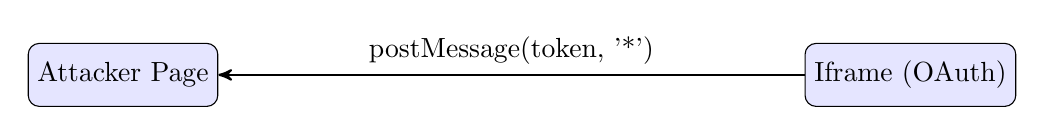
\begin{tikzpicture}[node distance=10cm, auto]
    \node[actor] (attacker) {Attacker Page};
    \node[actor, right of=attacker] (iframe) {Iframe (OAuth)};
    \draw[arrow] (iframe) -- node[above] {postMessage(token, '*')} (attacker);
\end{tikzpicture}


\subsubsection{Impact}
Token theft.

\subsubsection{Detection Methodology}
\begin{itemize}
    \item Check the JavaScript code for \texttt{postMessage} calls.
    \item Look for wildcard origins.
\end{itemize}


\subsubsection{Prevention}
\begin{itemize}
    \item Always specify the exact target origin in \texttt{postMessage}.
    \item Validate the origin of incoming messages.
\end{itemize}


% ---------------------------------------------------------------------
\section{OAuth Pentesting Methodology}
\subsection{Reconnaissance}
\begin{itemize}
    \item Identify OAuth endpoints:\\ \texttt{/.well-known/oauth-authorization-server}, \texttt{/.well-known/openid-configuration}.
    \item Find client IDs and redirect URIs from source code or network traffic.
    \item Determine supported grant types.
\end{itemize}

\subsection{Mapping the Flow}
\begin{itemize}
    \item Step through the OAuth flow with Burp proxy.
    \item Note parameters: \texttt{client\_id}, \texttt{redirect\_uri}, \texttt{response\_type}, \texttt{scope}, \texttt{state}.
    \item Identify all endpoints involved.
\end{itemize}

\subsection{Testing Redirect URI Validation}
\begin{itemize}
    \item Modify \texttt{redirect\_uri} to different domains.
    \item Use path traversal, subdomain variants, open redirects.
    \item Observe if code/token is leaked.
\end{itemize}

\subsection{Testing State Parameter}
\begin{itemize}
    \item Remove \texttt{state} and see if flow still works.
    \item Predict \texttt{state} if generated from session IDs or timestamps.
    \item Attempt CSRF by using a crafted URL.
\end{itemize}

\subsection{Testing Scope Validation}
\begin{itemize}
    \item Capture token exchange and modify scope.
    \item Test if token grants expanded permissions.
\end{itemize}

\subsection{Testing Token Leakage}
\begin{itemize}
    \item Check referer headers for token.
    \item Test if token appears in logs, browser history, or postMessage.
\end{itemize}

\subsection{Testing Account Linking}
\begin{itemize}
    \item Attempt to link a social account to an existing account.
    \item Check if the linking is CSRF-protected.
\end{itemize}

\section{Prevention and Mitigation}
\begin{itemize}
    \item Use Authorization Code flow with PKCE for public clients.
    \item Strictly validate \texttt{redirect\_uri} with exact matching.
    \item Always use a cryptographically random \texttt{state} parameter and validate it.
    \item Validate scope consistency during token exchange.
    \item Use OpenID Connect for authentication with proper ID token validation.
    \item Keep client secrets secure; use OAuth 2.0 for server-side apps only.
    \item Implement token revocation and short-lived tokens.
    \item Use introspection endpoints to validate tokens.
\end{itemize}

\section{Checklist for Penetration Testers}
\begin{enumerate}
    \item Identify all OAuth endpoints and grant types.
    \item Enumerate client IDs and registered redirect URIs.
    \item Test \texttt{redirect\_uri} validation:
        \begin{itemize}
            \item Change domain.
            \item Change path.
            \item Add extra parameters.
            \item Use path traversal.
            \item Use open redirect endpoints.
        \end{itemize}
    \item Test \texttt{state} parameter:
        \begin{itemize}
            \item Remove it.
            \item Use a predictable value.
            \item Test CSRF by forcing victim.
        \end{itemize}
    \item Test scope validation:
        \begin{itemize}
            \item Modify scope in token exchange.
            \item Verify token permissions.
        \end{itemize}
    \item Test token leakage:
        \begin{itemize}
            \item Check referer header.
            \item Check browser history.
            \item Check postMessage usage.
        \end{itemize}
    \item Test account linking:
        \begin{itemize}
            \item Attempt to link an account with CSRF.
            \item Attempt to link without verification.
        \end{itemize}
    \item Test for unverified user registration on the OAuth provider.
    \item Test client secret exposure (if applicable).
    \item Test for authorization server confusion (multiple issuers).
\end{enumerate}



\end{document}